% XCircuit output "RC_filter.tex" for LaTeX input from RC_filter.eps
\def\putbox#1#2#3#4{\makebox[0in][l]{\makebox[#1][l]{}\raisebox{\baselineskip}[0in][0in]{\raisebox{#2}[0in][0in]{\scalebox{#3}{#4}}}}}
\def\rightbox#1{\makebox[0in][r]{#1}}
\def\centbox#1{\makebox[0in]{#1}}
\def\topbox#1{\raisebox{-0.60\baselineskip}[0in][0in]{#1}}
\def\midbox#1{\raisebox{-0.20\baselineskip}[0in][0in]{#1}}
   \scalebox{0.626427}{
   \normalsize
   \parbox{2.29688in}{
   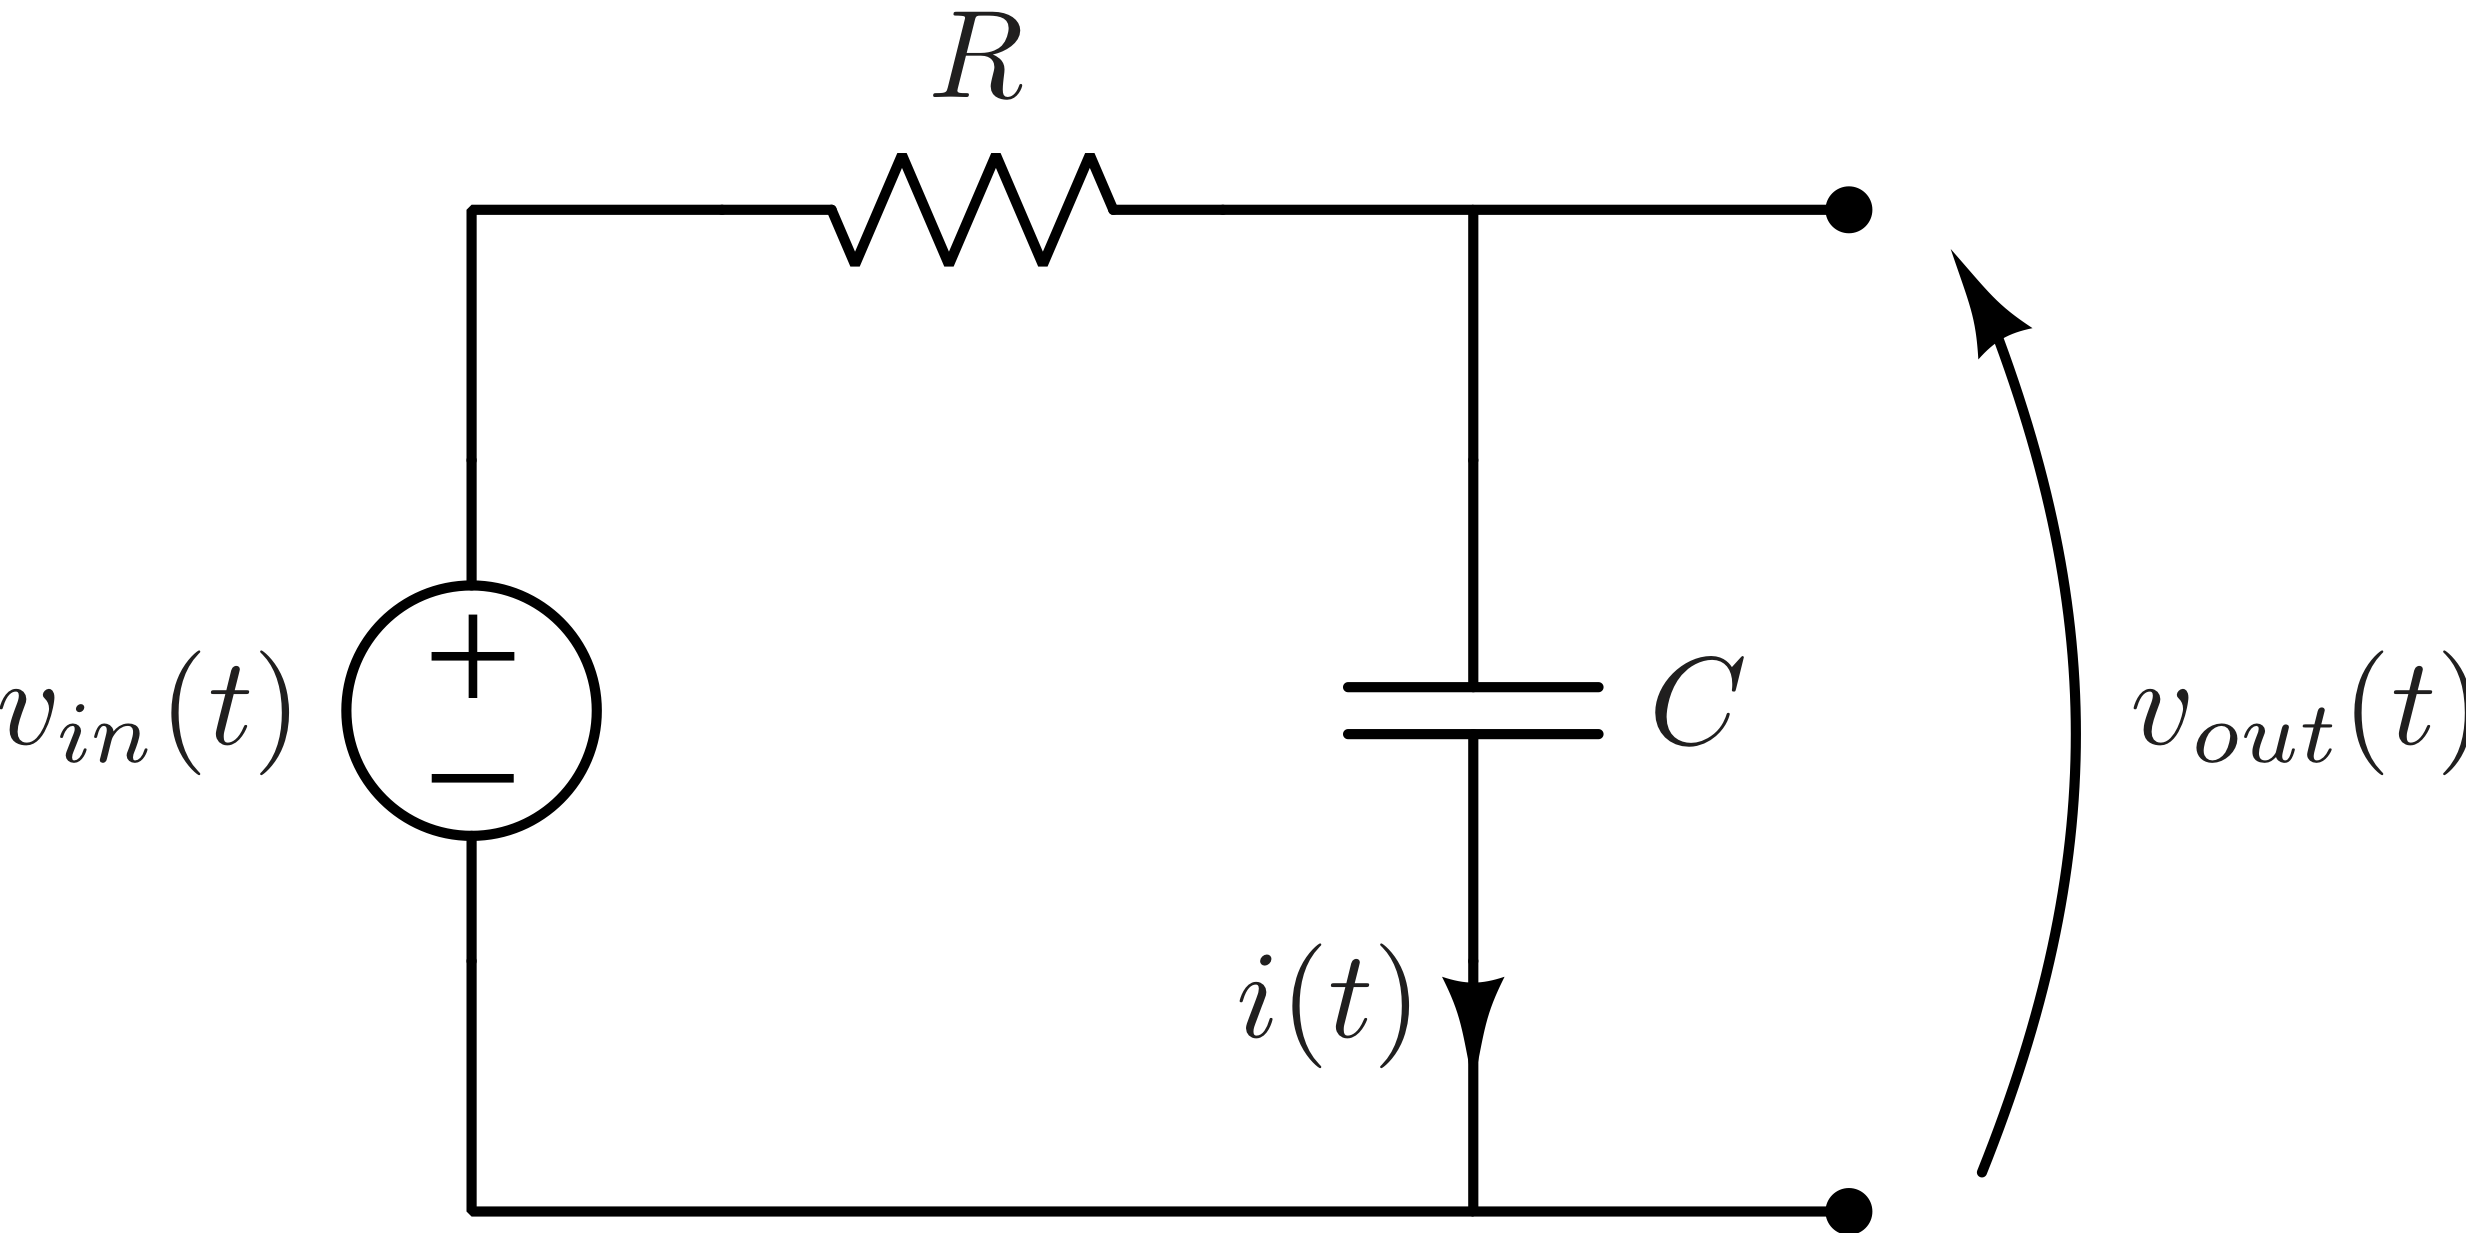
\includegraphics[scale=1.59635]{RC_filter}\\
   % translate x=498 y=408 scale 0.23
   \putbox{-0.38in}{0.74in}{1.20}{$v_{in}(t)$}%
   \putbox{0.86in}{1.6in}{1.20}{$R$}%
   \putbox{1.82in}{0.74in}{1.20}{$C$}%
   \putbox{2.46in}{0.74in}{1.20}{$v_{out}(t)$}%
   \putbox{1.27in}{0.35in}{1.20}{$i(t)$}%
   } % close 'parbox'
   } % close 'scalebox'
   \vspace{-\baselineskip} % this is not necessary, but looks better
